\subsection{Data Normalization}


\begin{figure}[H]
\centering
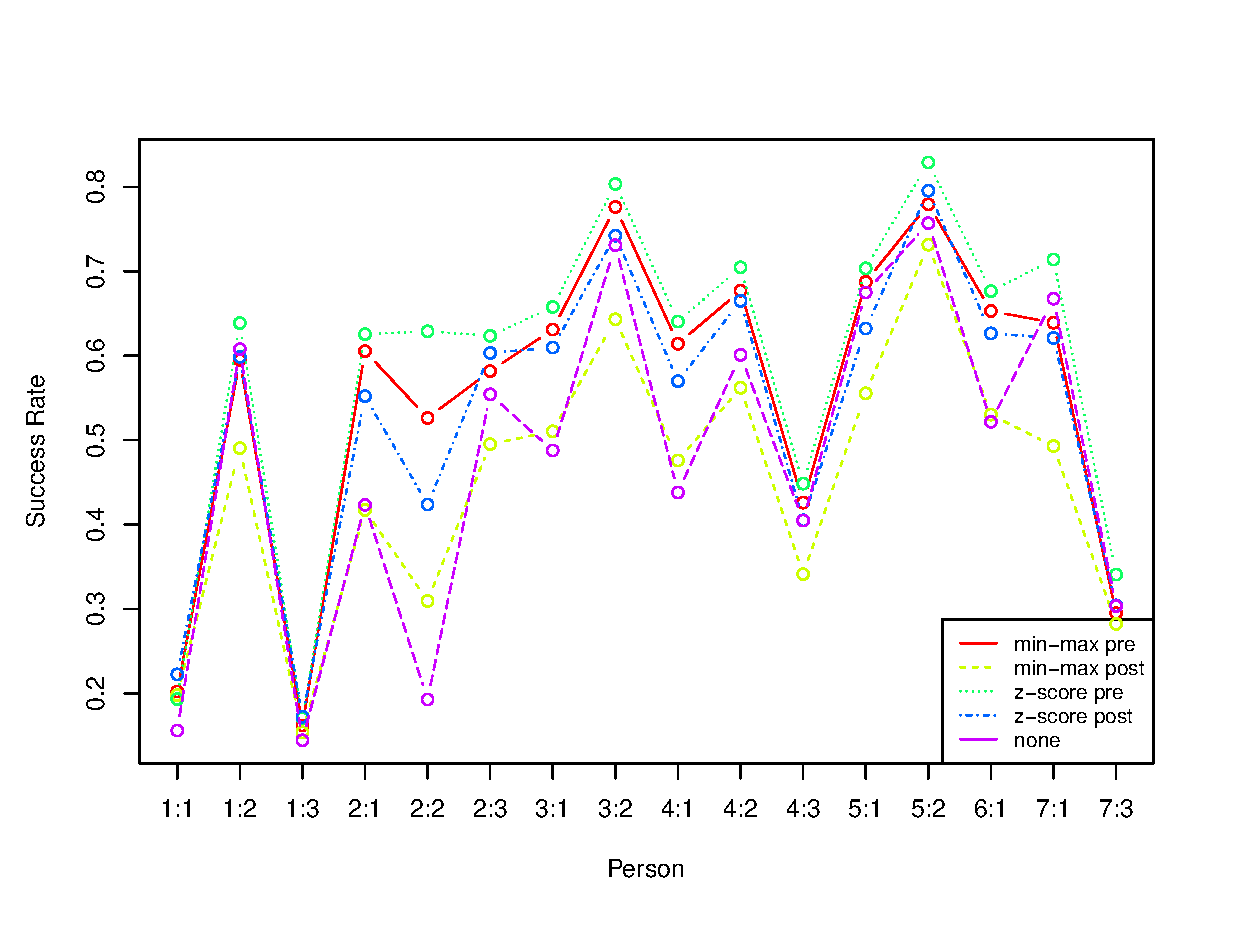
\includegraphics[width = 16cm]{graphics/graph_normalization_allppl}
\caption{Success rate for detection of characters of on person when not in the training set. 
Data normalized before (pre) and after (post) dataset reduction using PCA.
PCA was set to ensure that 80\% of all variance was included in the data set and K as 19.
The person tested for is given as 'Group':'Member'.
It was tested with 16 people.}
\label{fig:normalization_test_pre-post}
\end{figure}

\begin{table}[H]
\centering
\begin{tabular}{|l|r|}\hline
% 0.5532031 0.4493750 0.5874687 0.5339844 0.4791094
Normalization Method & Mean Success \\ \hline
Min-Max Normalization Pre & 55.3 \% \\ \hline
Min-Max Normalization Post & 44.9 \% \\ \hline
Z-Score Normalization Pre & 58.7 \% \\ \hline
Z-Score Normalization Post & 53.4  \% \\ \hline
No Normalization & 47.9 \% \\ \hline
\end{tabular}
\caption{}
\label{tab:meanSuccess_normalization_test_pre-post}
\end{table}

\begin{figure}
\centering
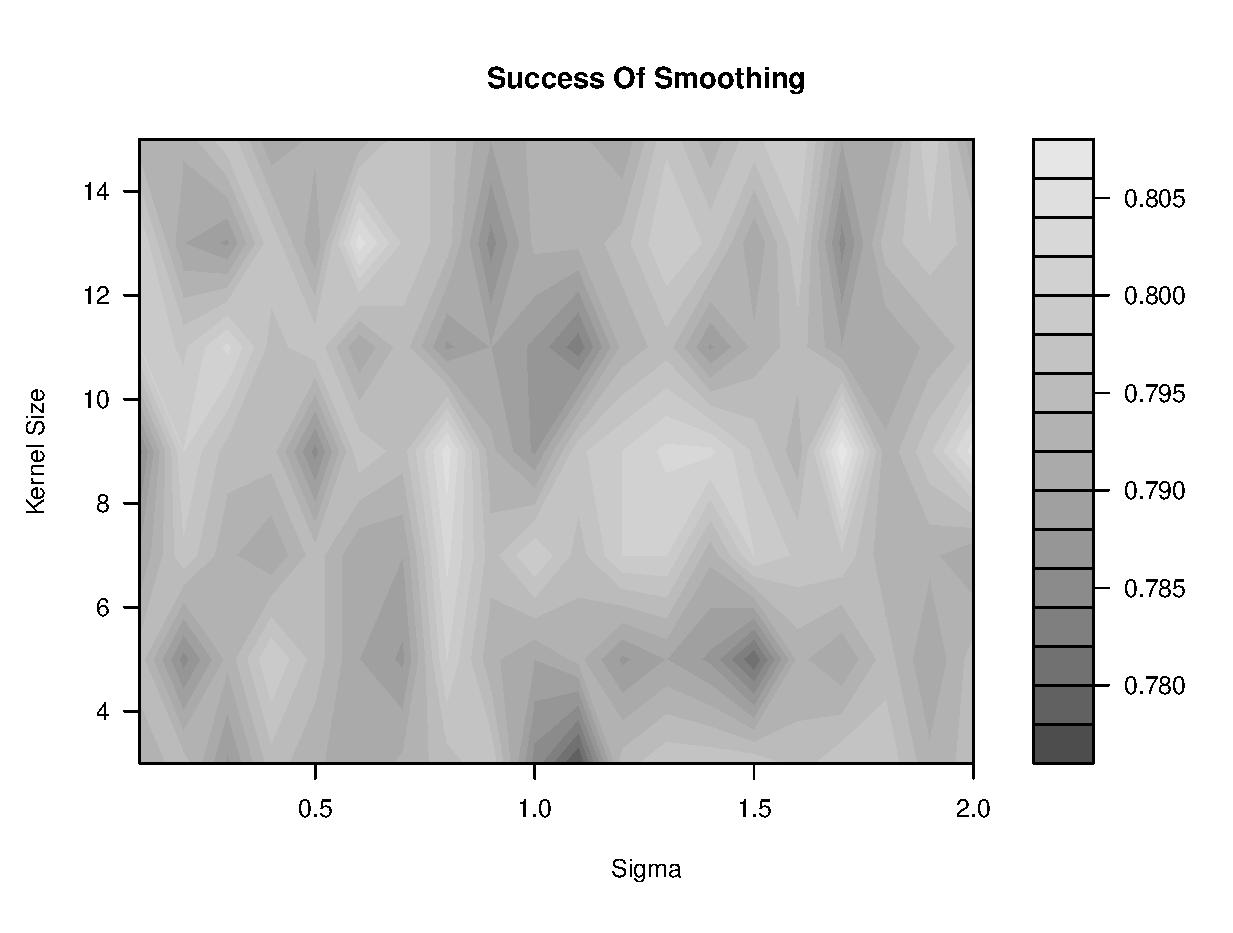
\includegraphics[width = \textwidth]{graphics/success_of_smoothing_contour}
\caption{To find the optimal kernel size the success detection rate was plotted with a varying $\sigma$.
The data was tested with group 3 member 2's data against 14 other students and preprocessed with a Gaussian filter. 
The optimal kernel size is chosen to be 9 pixels wide.
}
\end{figure}
